\documentclass[12pt]{article}
\usepackage[
backend=biber,
style=abnt,
sorting=nyt
]{biblatex}
\usepackage{csquotes}
\addbibresource{bibliografia.bib}
\AtBeginBibliography{\raggedright \footnotesize}
\setlength{\bibitemsep}{\baselineskip}

\usepackage{amsmath} %Para usar símbolos matemáticos

\usepackage[brazil]{babel} %Para usar a linguagem português
\addto\captionsbrazil{
    \renewcommand{\contentsname}{\texorpdfstring{\normalsize SUMÁRIO}{SUMÁRIO}}
    \renewcommand{\listtablename}{\texorpdfstring{\normalsize ÍNDICE DE TABELAS}{ÍNDICE DE TABELAS}}
    \renewcommand{\listfigurename}{\texorpdfstring{\normalsize ÍNDICE DE FIGURAS}{ÍNDICE DE FIGURAS}}
}

\usepackage{subcaption}
\usepackage{float}
\usepackage{graphicx} %Para inserir imagens
\usepackage{geometry} %Para alterar propriedades da página
\geometry{
a4paper,
left=30mm,
top=30mm,
right=20mm,
bottom=20mm
}

\usepackage[hidelinks]{hyperref}

\usepackage{tocloft}
\renewcommand{\cfttoctitlefont}{\hfill}
\renewcommand{\cftaftertoctitle}{\hfill}
\renewcommand{\cftsecfont}{\normalsize\normalfont\bfseries}
\renewcommand{\cftsubsecindent}{0pt}
\renewcommand{\cftsubsecfont}{\normalsize\normalfont}
\renewcommand{\cftsubsubsecindent}{0pt}
\renewcommand{\cftsubsubsecfont}{\normalsize\normalfont\bfseries}
\renewcommand{\cftsecleader}{\cftdotfill{\cftdotsep}}
\renewcommand{\cftlottitlefont}{\hfill} %Centralizar o título da lista de tabelas
\renewcommand{\cftafterlottitle}{\hfill}
\renewcommand{\cfttabpresnum}{Tabela\ } %Adicionar Tabela antes do nome de cada item
\renewcommand{\cfttabaftersnum}{:\ }
\setlength{\cfttabnumwidth}{4.75em}
\renewcommand{\cftdotsep}{1}
\renewcommand{\cftloftitlefont}{\hfill}
\renewcommand{\cftafterloftitle}{\hfill}
\renewcommand{\cftfigpresnum}{Figura\ }
\renewcommand{\cftfigaftersnum}{:\ }
\setlength{\cftfignumwidth}{4.75em}

\usepackage{titlesec}
\titleformat{\section}{\normalsize\bfseries\MakeUppercase}{\thesection}{0.5em}{}
\titleformat{\subsection}{\normalsize\MakeUppercase}{\thesubsection}{0.5em}{}
\titleformat{\subsubsection}{\normalsize\bfseries}{\thesubsubsection}{0.5em}{}

\usepackage{fancyhdr}
\pagestyle{fancy}
\fancyhf{} % Limpa os cabeçalhos e rodapés
\fancyhead[R]{\footnotesize\thepage} % Coloca o número da página no canto superior direito
\fancyfoot[C]{} % Remove qualquer número de página no rodapé
\renewcommand{\headrulewidth}{0pt} % Remove a linha horizontal do cabeçalho
\renewcommand{\footrulewidth}{0pt} % Remove a linha horizontal do rodapé

\usepackage{multicol}
\usepackage{pgfplots}
\pgfplotsset{compat=1.18}
\usepackage[american]{circuitikz}
\usetikzlibrary{external}\tikzexternalize
\usetikzlibrary{positioning}

\usepackage{setspace} %Para alterar o espaçamento das linhas
\setstretch{1.5}

\begin{document}
    \begin{titlepage}
    \begin{center}
        \large
        Universidade Federal do Espírito Santo - UFES\\
        Departamento de Computação e Eletrônica - DCEL\\
        Engenharia de Computação
        
        \vfill
        \textbf{
        Relatório da experiência 01\\
        Resistores\\~\\
        }
        
        Disciplina: Circuitos Elétricos I\\
        Prof. Flávio Duarte Couto Oliveira\\
        
        \vfill
        \begin{flushright}
            Pedro Henrique Alves do Nascimento
        \end{flushright}
        
        \vfill
        Espírito Santo\\
        Dezembro 2024
    \end{center}
    \newpage
\end{titlepage}
    
    \listoftables
    \thispagestyle{empty}
    \newpage

    \listoffigures
    \thispagestyle{empty}
    \newpage

    \tableofcontents
    \thispagestyle{empty}
    \newpage

    \section*{Pedro Henrique Alves do Nascimento}
    \section{INTRODUÇÃO TEÓRICA}
    \subsection{LEI DE OHM}\indent
    
    A lei de Ohm é a relação algébrica entre corrente tensão para um resistor \parencite{nilsson}, dada pela Equação \ref{lei-de-ohm}
    \begin{equation}
        V=R\times i \label{lei-de-ohm}
    \end{equation}
    onde $V$ é a tensão, em Volts (V) nos terminais do resistor, $R$ é a resistência elétrica do resistor, em Ohms ($\Omega$) e $i$ a corrente que passa pelo resistor, em Ampères (A).

    Ou seja, traçando-se um gráfico de tensão $\times$ corrente para um resistor ôhmico, tem-se uma função linear, onde $\tan{\alpha}=\frac{V'}{i'}$ é a resistência $R$ daquele resistor, como mostrado na Figura \ref{fig:resistorohmico}.
        \begin{figure}[h!]
            \centering
            \begin{minipage}{0.5\textwidth}
                \centering
                \caption{Gráfico $V\times i$ de um resistor ôhmico.}
                \begin{tikzpicture}
                    \begin{axis}[
                        axis lines=middle,
                        xlabel={$i$},
                        ylabel={$V$},
                        xmin=-0.5, xmax=3,
                        ymin=-0.5, ymax=3,
                        xtick={1.15},
                        xticklabel={$i'$},
                        ytick={2},
                        yticklabel={$V'$}
                    ]
                    \addplot[
                        thick,
                        domain=0:2,
                        samples=5,
                    ] {sqrt(3)*x};
                    \draw[smooth, thick] (0.5,0) arc (0:60:0.5) node[midway] {$\alpha$};
                    \node at (axis cs:0,0) [anchor=north east] {$0$};
                    \draw[dashed, color=gray!50] (0,2) -- (1.15,2) -- (1.15,0);
                    \end{axis}
                \end{tikzpicture}

                \raggedright \footnotesize Fonte: Elaborado pelo autor.
                \label{fig:resistorohmico}
            \end{minipage}
        \end{figure}
    
    \subsection{RESISTORES}\indent

    Resistores são componentes eletrônicos projetados para limitar a passagem de corrente elétrica em um circuito, transformando parte da energia elétrica em calor, e são geralmente feitos de materiais com alta resistividade, como carbono ou filme metálico. Os resistores podem ser classificados em fixos (resistência constante) e variáveis (resistência que pode ser alterada).

    Os resistores fixos têm suas propriedades, valor nominal e tolerância, classificadas conforme uma tabela de cores indicada na Tabela \ref{tab:corResist}.
    
    \begin{figure}[H]
        \centering
        \begin{minipage}{0.5\textwidth}
            \centering
            \caption{Resistor e suas faixas.}
            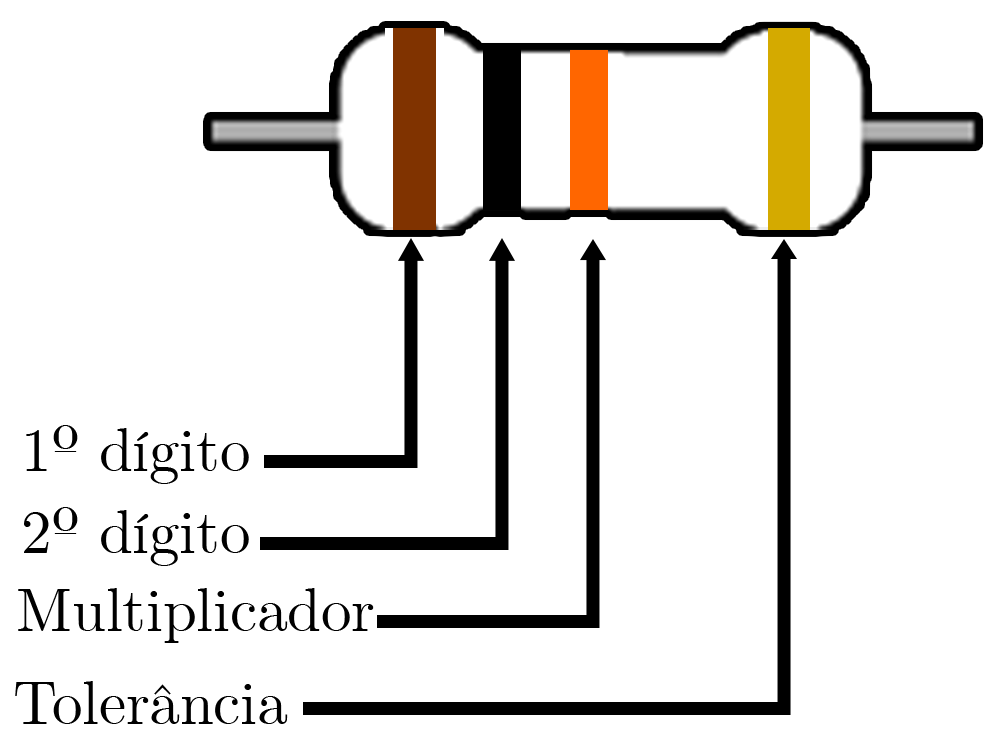
\includegraphics[width=\textwidth]{external-figures/cores-resistores.png}
            \raggedright \footnotesize Fonte: kitsarduino.com.br (Adaptado).
            \label{fig:resistor}
        \end{minipage}
    \end{figure}
    \begin{table}
        \caption{Tabela do cores dos resistores fixos.}
        \label{tab:corResist}
        \centering
        \vspace{0.5em}
        \setstretch{1.5}{
        \begin{tabular}{ccclc}
        \hline
        Cor & 1ª Faixa & 2ª Faixa & Multiplicador ($\Omega$) & Tolerância\\
        \hline Preto & 0 & 0 & $\times 1$ & \\
        Marrom & 1 & 1 & $\times 10$ & $\pm$ 1\%\\
        Vermelho & 2 & 2 & $\times 100$ & $\pm$ 2\%\\
        Laranja & 3 & 3 & $\times 1$ k & \\
        Amarelo & 4 & 4 & $\times 10$ k & \\
        Verde & 5 & 5 & $\times 100$ k & $\pm$ 0.5\%\\
        Azul & 6 & 6 & $\times 1$ M & $\pm$ 0.25\%\\
        Violeta & 7 & 7 & $\times 10$ M & $\pm$ 0.1\%\\
        Cinza & 8 & 8 & & $\pm$ 0.05\%\\
        Branco & 9 & 9 & & \\
        Dourado & & & $\times 0.1$ & $\pm$ 5\%\\
        Prateado & & & $\times 0.01$ & $\pm$ 10\%\\
        \hline
        \end{tabular}}\\
        \footnotesize Fonte: blog.fazedores.com (Adaptado)\nocite{codigo_cores_resistores}.
    \end{table}

    Resistores variáveis possuem três terminais, a resistência desejada é obtida variando a posição do terminal central em relação aos mais externos, a resistência máxima é obtida quando o terminal central está na posição 3. Um exemplo de potenciômetro é mostrado na Figura \ref{fig:potenciometro}.

    \begin{figure}[H]
        \centering
        \begin{minipage}{0.4\textwidth}
            \centering
            \caption{Representação gráfica de potenciômetro.}
            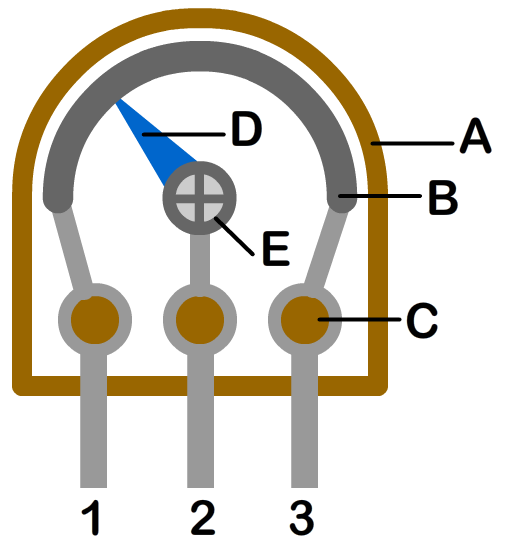
\includegraphics[width=\textwidth]{external-figures/resistor-variavel.png}
            \raggedright \footnotesize Fonte: ricardoteix.com.
            \label{fig:potenciometro}
        \end{minipage}
    \end{figure}
    
    Esse funcionamento advém da variação do comprimento do segmento do resistor, que, pela equação $R = \rho\times\frac{L}{A}$ --- onde $R$ é a resistência do material, $\rho$ a sua resistividade, $L$ o comprimento e $A$ a área da seção transversal --- é diretamente proporcional ao comprimento do resistor, ou seja, quanto mais próximo do terminal 3, maior a resistência obtida.

    Alguns usos de resistores variáveis se dão em equipamentos de áudio, onde o volume, por exemplo, depende diretamente da tensão.
    \begin{figure}[H]
        \centering
        \caption{Representação de resistor fixo e variável em um circuito.}
        \begin{tikzpicture}
            \draw (-0.5,0) -- (0,0) to [R, label=$R$] (1,0) -- (1.5,0) to
            [open] (2.5,0) -- (3,0) to
            [vR, l=$R_{var}$] (4,0) -- (4.5,0);
        \end{tikzpicture}
    \end{figure}
    

    \subsection{OHMÍMETRO}\indent
    Ohmímetros são equipamentos de medição de resistência elétrica.
    
    Teste 2.
    \begin{figure}[h!]
        \centering
        \begin{minipage}{0.5\textwidth}
            \centering
            \caption{Descrição da figura.}
            \includegraphics[width=\textwidth]{example-image}
            \raggedright \footnotesize Fonte: Autor ou fonte da imagem.
            \label{fig:minhaFigura}
        \end{minipage}
    \end{figure}
\newpage
Teste circuitos:

\begin{tikzpicture}
    \draw (0,0) -- (1,0);
\end{tikzpicture}

\begin{center}\small
    \begin{circuitikz}[american]
        \draw (0,0) to [resistor, l=10 $\Omega$] (3,0) to [short, *-] (3,0)
        to [resistor, l_=60 $\Omega$] (3,2)
        to [resistor, l_=10 $\Omega$] (3,4)
        to [resistor, l_=130 $\Omega$] (3,6)
        to [short, *-, f_<=$i_g$] (0,6)
        to [voltage source, v_=600 V, sources/scale=2] (0,0);
        \draw (3,6) to [R, l=34 $\Omega$] (7,6)
        to [short, *-] (7,6)
        to [R, l=72 $\Omega$, f_=$i_0$] (7,3)
        to [R, l=8 $\Omega$] (7,0)
        to [short, -*] (7,0)
        to (7,0) -- (3,0);
        \draw (7,6) to (7,6) -- (10,6)
        to [R, l=20 $\Omega$] (10,0)
        to (10,0) -- (7,0);
    \end{circuitikz}
\end{center}

\begin{center}
\Large
\begin{circuitikz}[scale=0.5, transform shape]
    \node (A) at (6.5,3) {};
    \node (B) at (8.5,3) {};
    \ctikzset{nodes width=0.08};
    \draw(0,0) to [short, -*] (3,0)
    to [R, l_=3 k$\Omega$, -*] (3,3)
    to [R, l_=2 k$\Omega$, -*] (3,6)
    to [short] (0,6)
    to [current source, l_=4.5 mA, invert, sources/scale=2] (0,0);
    \draw (3,6) to [short] (12,6)
    to [R, l=1.5 k$\Omega$, -*] (12,3)
    to [R, l=6 k$\Omega$] (12,0)
    to [short] (3,0);
    \draw (3,3) to [R, l=1 k$\Omega$, -*] (A) node[label={above: +}] {};
    \draw (12,3) to [R, l_=5 k$\Omega$, -*] (B) node[label={above: -}] {};
    \draw (A) to [open, l=$v_0$] (B);
\end{circuitikz}
\end{center} 


Isso está na figura \ref{fig:minhaFigura}. Segue a equação \ref{eq: Potência} da Potência:
    \begin{multicols}{2}
        
        \begin{equation}
            P = \frac{dw}{dt}
            \label{eq: Potência}
        \end{equation}
        \columnbreak
        
        \noindent $P$ = Potência, em Watts\\
        $w$ = Trabalho, em Joules\\
        $t$ = Tempo, em segundos\\
    \end{multicols}
    
\begin{table}[H]
    \centering
    \caption{Sample Table 1}
    \begin{tabular}{|c|c|}
        \hline
        Column 1 & Column 2 \\
        \hline
        Data 1 & Data 2 \\
        \hline
    \end{tabular}
    \label{tab:tabela teste}
\end{table}

\begin{table}[H]
    \centering
    \caption{Sample Table 2}
    \begin{tabular}{|c|c|}
        \hline
        Column A & Column B \\
        \hline
        Data A & Data B \\
        \hline
    \end{tabular}
\end{table}

\parencite{einstein}
\cite{dirac}

\newpage
\setstretch{1}
\section*{\hfill REFERÊNCIAS BIBLIOGRÁFICAS\hfill}
\addcontentsline{toc}{section}{REFERÊNCIAS BIBLIOGRÁFICAS}
\printbibliography[heading=none]
\end{document}